\documentclass[border=6pt,tikz]{standalone}
\usepackage{tikz}
\usepackage{amsmath,amssymb}
\usetikzlibrary{arrows.meta,positioning,fit,backgrounds,calc,shapes.geometric,decorations.pathreplacing,patterns}
\definecolor{ink}{HTML}{1B2430}
\definecolor{muted}{HTML}{6B7785}
\definecolor{accent}{HTML}{2F6FB5}
\definecolor{accent2}{HTML}{C1611F}
\definecolor{good}{HTML}{2E7D5B}
\definecolor{soft}{HTML}{EDF2F7}
\definecolor{soft2}{HTML}{FBEDE2}
\definecolor{soft3}{HTML}{E6F0E9}
\tikzset{
  box/.style={draw=ink,line width=.7pt,rounded corners=2pt,fill=soft,inner sep=4pt,align=center,font=\sffamily\small},
  boxa/.style={box,fill=soft2},
  boxb/.style={box,fill=soft3},
  plain/.style={align=center,font=\sffamily\small,text=ink},
  tiny/.style={align=center,font=\sffamily\scriptsize,text=muted},
  ar/.style={-{Stealth[length=2.4mm]},draw=ink,line width=.7pt},
  arm/.style={-{Stealth[length=2.4mm]},draw=muted,line width=.6pt,dashed},
  nd/.style={circle,draw=ink,line width=.7pt,fill=white,minimum size=7mm,inner sep=0pt,font=\sffamily\scriptsize},
  ndf/.style={nd,fill=soft},
  ndt/.style={nd,fill=soft2},
}

\begin{document}
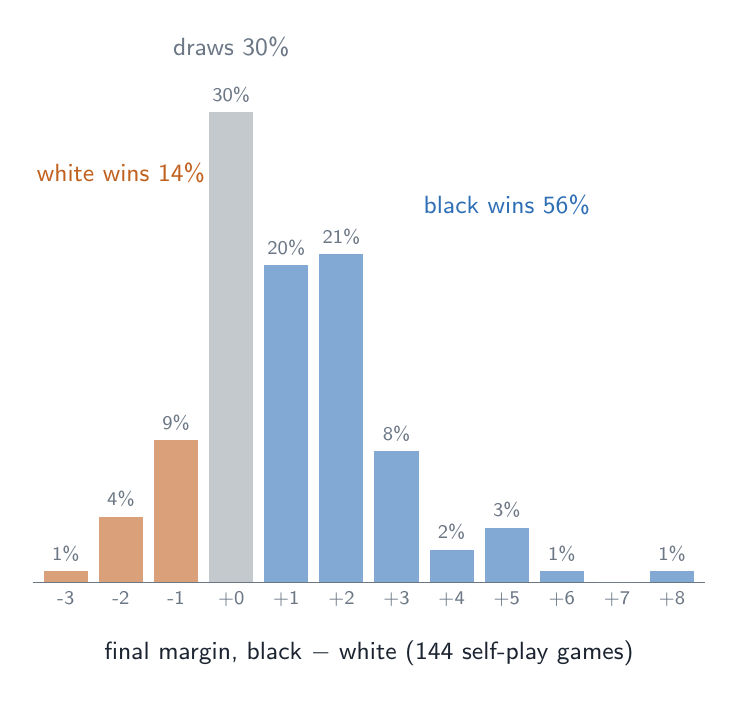
\begin{tikzpicture}[x=7mm,y=2mm]
\draw[muted,line width=.3pt] (-3.6,0) -- (8.6,0);
\fill[accent2!60] (-3.4,0) rectangle (-2.6,0.69);
\node[tiny,above] at (-3,0.69) {1\%};
\node[tiny,below] at (-3,0) {-3};
\fill[accent2!60] (-2.4,0) rectangle (-1.6,4.17);
\node[tiny,above] at (-2,4.17) {4\%};
\node[tiny,below] at (-2,0) {-2};
\fill[accent2!60] (-1.4,0) rectangle (-0.6,9.03);
\node[tiny,above] at (-1,9.03) {9\%};
\node[tiny,below] at (-1,0) {-1};
\fill[muted!40] (-0.4,0) rectangle (0.4,29.86);
\node[tiny,above] at (0,29.86) {30\%};
\node[tiny,below] at (0,0) {+0};
\fill[accent!60] (0.6,0) rectangle (1.4,20.14);
\node[tiny,above] at (1,20.14) {20\%};
\node[tiny,below] at (1,0) {+1};
\fill[accent!60] (1.6,0) rectangle (2.4,20.83);
\node[tiny,above] at (2,20.83) {21\%};
\node[tiny,below] at (2,0) {+2};
\fill[accent!60] (2.6,0) rectangle (3.4,8.33);
\node[tiny,above] at (3,8.33) {8\%};
\node[tiny,below] at (3,0) {+3};
\fill[accent!60] (3.6,0) rectangle (4.4,2.08);
\node[tiny,above] at (4,2.08) {2\%};
\node[tiny,below] at (4,0) {+4};
\fill[accent!60] (4.6,0) rectangle (5.4,3.47);
\node[tiny,above] at (5,3.47) {3\%};
\node[tiny,below] at (5,0) {+5};
\fill[accent!60] (5.6,0) rectangle (6.4,0.69);
\node[tiny,above] at (6,0.69) {1\%};
\node[tiny,below] at (6,0) {+6};
\fill[accent!60] (6.6,0) rectangle (7.4,0.00);
\node[tiny,below] at (7,0) {+7};
\fill[accent!60] (7.6,0) rectangle (8.4,0.69);
\node[tiny,above] at (8,0.69) {1\%};
\node[tiny,below] at (8,0) {+8};
\node[plain] at (2.5,-4.5) {final margin, black $-$ white (144 self-play games)};
\node[plain,text=accent2] at (-2,26) {white wins 14\%};
\node[plain,text=muted] at (0,34) {draws 30\%};
\node[plain,text=accent] at (5,24) {black wins 56\%};
\end{tikzpicture}
\end{document}
